\documentclass{standalone}
\usepackage{amsmath,mathabx}
\usepackage{tikz}
\usetikzlibrary{positioning}
\begin{document}
    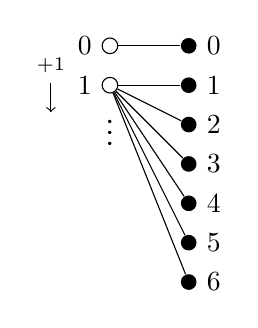
\begin{tikzpicture}[scale=0.5]
        %white
        \node[fill=white,draw =black, circle, inner sep=2pt, label=left:{\textcolor{black}{$0$}}] (w0) at (0,0) {};
        \node[fill=white,draw = black, circle, inner sep=2pt, label=left:{\textcolor{black}{$1$}}] (w1) at (0,-1) {};
        \node at (0,-2) {\large $\vdots$};

        %\node[draw=black, fill=white, circle, inner sep=1pt] (circ) at (-1.5,-0.5) {};
        \node (p1) at (-1.5,-0.5) {\scriptsize +1};
        \draw[->] ([yshift=0pt] p1.south) -- ++(0, -0.75);
        %black nodes
        \node[fill=black, circle, inner sep=2pt, label=right:{\textcolor{black}{$0$}}] (b0) at (2,0) {};
        \node[fill=black, circle, inner sep=2pt, label=right:{\textcolor{black}{$1$}}] (b1) at (2,-1) {};
        \node[fill=black, circle, inner sep=2pt, label=right:{\textcolor{black}{$2$}}] (b2) at (2,-2) {};
        \node[fill=black, circle, inner sep=2pt, label=right:{\textcolor{black}{$3$}}] (b3) at (2,-3) {};
        \node[fill=black, circle, inner sep=2pt, label=right:{\textcolor{black}{$4$}}] (b4) at (2,-4) {};
        \node[fill=black, circle, inner sep=2pt, label=right:{\textcolor{black}{$5$}}] (b5) at (2,-5) {};
        \node[fill=black, circle, inner sep=2pt, label=right:{\textcolor{black}{$6$}}] (b6) at (2,-6) {};
        \node at (0,-2) {\large $\vdots$};

        \draw[draw=black, shorten >=0pt, shorten <=0pt] (w0) -- (b0);
        \draw[draw=black, shorten >=0pt, shorten <=0pt] (w1) -- (b1);
        \draw[draw=black, shorten >=0pt, shorten <=0pt] (w1) -- (b2);
        \draw[draw=black, shorten >=0pt, shorten <=0pt] (w1) -- (b3);
        \draw[draw=black, shorten >=0pt, shorten <=0pt] (w1) -- (b4);
        \draw[draw=black, shorten >=0pt, shorten <=0pt] (w1) -- (b5);
        \draw[draw=black, shorten >=0pt, shorten <=0pt] (w1) -- (b6);
    \end{tikzpicture}
\end{document}